\documentclass[]{imag-ms-template}

%the class loads mathtools, amssymb, booktabs, graphicx, biblatex (APA, natbib commands) and hyperref
\usepackage[utf8]{inputenc}
\usepackage[T1]{fontenc}
\usepackage{lmodern}
\IfFileExists{microtype.sty}{\usepackage{microtype}}{}
\usepackage{multirow}
\usepackage{xcolor}
\usepackage{tikz}
\usetikzlibrary{calc,decorations.pathreplacing,calligraphy,shapes.geometric,intersections}
\usepackage{caption}
\usepackage{subcaption}
\usepackage{placeins}
\usepackage{lineno}
\usepackage{xr}
\externaldocument[M-]{main}
\linenumbers
\hypersetup{colorlinks=true,linkcolor=blue!50!black,citecolor=blue!50!black,urlcolor=blue!50!black}
\addbibresource{references.bib}

%points the authors must check before submission
\newcommand{\TBD}[1]{\textcolor{red}{[#1]}}
\newcommand{\E}{\mathbb{E}}
\newcommand{\R}{\mathbb{R}}
%\input is not expandable inside tabular (misplaced \noalign before \bottomrule); the TeX primitive is
\makeatletter\newcommand{\tabinput}[1]{\@@input #1.tex }\makeatother
%auto-generated by make_tables.py; do not edit
\newcommand{\ridgeEEGvsECG}{0.00}
\newcommand{\ridgeEEGvsMOTION}{0.02}
\newcommand{\ridgeEEGvsHR}{0.64}

%auto-generated by make_tables.py; do not edit
\newcommand{\sesoiNLL}{0.104}
\newcommand{\sesoiCRPS}{0.011}
\newcommand{\sesoiRMSE}{0.023}


\renewcommand{\thesection}{S\arabic{section}}
\renewcommand{\thetable}{S\arabic{table}}
\renewcommand{\thefigure}{S\arabic{figure}}
\renewcommand{\theequation}{S\arabic{equation}}

\title{Supplementary Material for\\Is the Uncertainty About the EEG?\\Positive Controls and Physiological Confounds in EEG-to-fMRI Synthesis}

\author{David Calhas,$^{1\ast}$ Rui Henriques$^{2}$\\
{\small $^{1}$Faculty of Computer and Information Science, University of Ljubljana, Ljubljana, Slovenia}\\
{\small $^{2}$INESC-ID, Instituto Superior T\'{e}cnico, Universidade de Lisboa, Lisbon, Portugal}\\
{\small $^\ast$Correspondence: David Calhas, david.calhas@fri.uni-lj.si}
}
\date{}

\begin{document}
\maketitle

This document extends the main text. Section~\ref{supp:related} reviews related work in more detail, Section~\ref{supp:methods} gives the full methods, Section~\ref{supp:decoder} the construction of the stochastic spectral decoder, Section~\ref{supp:results} the complete results with all supplementary tables and figures, and Section~\ref{supp:discussion} an extended discussion. Figures and tables numbered without ``S'' refer to the main text.

\section{Extended related work}\label{supp:related}
\paragraph{EEG-to-fMRI synthesis.} EEG and BOLD are related through neurovascular coupling. Band-limited EEG power, alpha in particular, correlates with BOLD in specific networks \citep{goldman2002simultaneous,laufs2003eeg,mukamel2005coupling}, and resting-state connectomes covary across the two modalities \citep{deligianni2014relating}. \citet{liu2019convolutional} first trained a convolutional network to map EEG to fMRI volumes, and \citet{calhas2022eeg} proposed a topographical-attention encoder with a latent-space decoder. We use the latter as the backbone of every synthesizer in this study. More recent models predict region-level BOLD signals rather than volumes \citep{li2024neurobolt}. Sparse, lagged linear models on EEG band power predict region-of-interest BOLD within subjects beyond surrogate nulls \citep{mehta2025eegbold}; we run a model of this kind on our data (Section~\ref{sec:ridge}). To our knowledge no prior work has asked whether a synthesizer's \emph{uncertainty} depends on the EEG.

\paragraph{Uncertainty in deep regression.} \citet{kendall2017uncertainties} separated aleatoric uncertainty, modelled with an input-dependent likelihood scale, from epistemic uncertainty, modelled with a distribution over weights. Weight distributions are approximated by variational inference \citep{blundell2015weight}, with Flipout to decorrelate gradients within a batch \citep{wen2018flipout}, by MC dropout \citep{gal2016dropout}, by stochastic weight averaging (SWAG) \citep{maddox2019simple}, and by Laplace approximations \citep{daxberger2021laplace}. Deep ensembles \citep{lakshminarayanan2017simple} remain a strong baseline, including under dataset shift \citep{ovadia2019can}. Evidential regression predicts the parameters of a Normal-Inverse-Gamma prior and so obtains both kinds of uncertainty in a single pass \citep{amini2020deep}. Reviews of these methods are given by \citet{abdar2021review}.

\paragraph{Calibration and conformal prediction.} A predictive distribution is calibrated if its intervals cover the target at their nominal rate. Recalibration can enforce this after training \citep{kuleshov2018accurate}. Split conformal prediction gives finite-sample, distribution-free coverage when calibration and test units are exchangeable \citep{vovk2005algorithmic,lei2018distribution,angelopoulos2023gentle}. Conformalized quantile regression adapts the interval width to the input \citep{romano2019conformalized}, and conformal risk control has been extended to image-to-image regression \citep{angelopoulos2022image}. Proper scoring rules such as the NLL and the CRPS reward calibration and sharpness together \citep{gneiting2007strictly}. In medical imaging, calibration and uncertainty have been studied for segmentation \citep{mehrtash2020confidence}, MRI reconstruction and super-resolution \citep{narnhofer2021bayesian,zhang2019reducing} and diffusion MRI enhancement \citep{tanno2021uncertainty}. Like this paper, these works treat calibration as necessary. Unlike it, they predict targets that are mostly determined by the input image, so they need not ask whether the uncertainty depends on the input.

\paragraph{Spectral parametrizations.} The DCT \citep{ahmed1974discrete} underlies JPEG compression \citep{wallace1992jpeg}. Truncating it is a classical way to reduce the degrees of freedom of an image model, and spectral smoothing reduces gradient variance \citep{pervez2021spectral}. Dropout applied in the spectral domain has been used as a regularizer \citep{khan2019regularization}; we include it as a UQ method (MC spectral dropout). The von Mises distribution models the phases of spectral coefficients in audio source separation \citep{magron2018bayesian}, phase-aware speech enhancement \citep{gerkmann2014bayesian} and harmonic signal modelling \citep{kulmer2015harmonic}. Implicit reparameterization gradients make it usable in neural networks \citep{figurnov2018implicit}.

\paragraph{Negative controls in neuroimaging machine learning.} Small samples give large error bars in cross-validation \citep{varoquaux2018cross}, leakage inflates reported performance \citep{kapoor2023leakage}, and networks exploit shortcuts \citep{geirhos2020shortcut}. For EEG--BOLD coupling, surrogate time series that preserve the spectrum of the predictor are the standard null \citep{schreiber1996improved}. Head motion \citep{friston1996movement,power2014methods} and cardiac signals both affect BOLD and are recorded alongside the EEG, so both are natural confound controls. Our protocol transfers these practices to predictive uncertainty.


\section{Extended methods}\label{supp:methods}
\subsection{Data}
We use CHUR-XP2 (OpenNeuro ds002338) \citep{lioi2019simultaneous}: simultaneous EEG--fMRI from 17 healthy participants performing motor imagery with neurofeedback. We use the motor imagery run recorded after neurofeedback training (\texttt{MIpost}), a block design with the same timing for every participant. EEG was recorded with 64 channels (63 scalp electrodes in the 10--20 system and one ECG lead) at 5\,kHz. We use the dataset's preprocessed export, which is corrected for gradient and pulse artefacts, low-passed at 50\,Hz and resampled to 200\,Hz. fMRI was acquired with $\mathrm{TR}=1$\,s, $\mathrm{TE}=23$\,ms, $2\times2\times4$\,mm voxels and a $108\times108\times16$ matrix, and is resized to $64\times64\times30$ by a DCT low-pass in-plane and zero-filling along $z$. The target therefore has at most 16 non-trivial frequencies along $z$. We checked the EEG--fMRI alignment from the scanner markers: the EEG export starts within 0.06\,s of the first volume.

We do not use the resting-state NODDI dataset \citep{deligianni2014relating}: in its public export we could not pair EEG and fMRI from the scanner triggers for every subject, and the alignment check above is a requirement of our protocol. We replicate the main analyses on the motor-localizer run of CHUR-XP1 (ds002336; 9 subjects with an EEG export of that run, TR 2\,s, 32 slices), on registered volumes, with every 2-s EEG window aligned to its scanner pulse (Section~\ref{sec:res:xp1}).


\subsection{Problem formulation and scores}\label{supp:problem}
\paragraph{Data and task.} A dataset contains $S$ subjects. Subject $s$ has paired sequences $\{(x_{s,t}, y_{s,t})\}_{t=1}^{T_s}$, where $y_{s,t}\in\R^{V}$ is the fMRI volume acquired at time $t$ ($V = 64\times 64\times 30$ voxels) and $x_{s,t}\in\R^{C\times F\times W}$ is the short-time Fourier magnitude of the $C$ EEG channels over the $W$ seconds preceding it (so that it covers the haemodynamic delay). A synthesizer is a conditional predictive distribution $p_\theta(y\mid x)$ trained on a set of training subjects $\mathcal{S}_{\mathrm{tr}}$ and evaluated on disjoint test subjects $\mathcal{S}_{\mathrm{te}}$. A disjoint set of calibration subjects $\mathcal{S}_{\mathrm{cal}}$ is used for conformal calibration. All splits are by subject; no subject contributes volumes to two sets.

\paragraph{Scores.} For a test pair $(x,y)$ and a predictive distribution $p$ we use the voxel-averaged negative log-likelihood $\mathrm{NLL} = -\frac{1}{|B|}\sum_{v\in B}\log p(y_v\mid x)$ and the continuous ranked probability score $\mathrm{CRPS} = \frac{1}{|B|}\sum_{v\in B}\E|Y_v-y_v| - \tfrac12\E|Y_v-Y'_v|$ with $Y,Y'\sim p(\cdot\mid x)$ independent \citep{gneiting2007strictly}, both over a fixed brain mask $B$. We also use the brain RMSE of the predictive mean, the prediction interval coverage probability (PICP) and width of the central $\alpha$-intervals, Spearman's $\rho$ between the predictive standard deviation and the absolute error, and the area under the sparsification error curve (AUSE). The mask $B$ is the Otsu threshold \citep{otsu1979threshold} of the training subjects' mean volume, so it depends on no test data. Every score is first averaged over each test subject's volumes, and then over seeds; subjects, not volumes, are the unit of every test.

\paragraph{The EEG-conditional question.} The checks above evaluate $p_\theta(y\mid x)$ against $y$. They do not ask whether $p_\theta$ depends on $x$. We say that a synthesizer's predictive distribution is \emph{informative about the EEG} if it passes two comparisons.

\emph{(i) EEG-free references.} It must score better than predictive distributions that never see EEG:
\begin{itemize}
	\item the \textbf{population template} $p_0(y) = \prod_v \mathcal{N}(y_v; \bar m_v, \bar s_v^2)$, with the voxelwise mean and standard deviation of all training volumes;
	\item the \textbf{stimulus-locked template} $p_{\mathrm{lock}}(y\mid t) = \prod_v\mathcal{N}(y_v; \bar m_{v,t}, \bar s^2_{v,t})$, with moments over training subjects at the same volume index $t$. In a block design with the same timing for every subject, this template predicts the task-evoked response without any EEG;
	\item the \textbf{own-subject oracle} $p_{\mathrm{own}}(y) = \prod_v \mathcal{N}(y_v; m^{(s)}_v, (s^{(s)}_v)^2)$, with the moments of the test subject's own volumes. It uses test data and is an upper bound for any predictor that gets the subject's static image right and nothing else.
\end{itemize}
A method passes if its subject-level NLL and CRPS are lower than those of $p_0$ and $p_{\mathrm{lock}}$, by a one-sided Wilcoxon signed-rank test over test subjects \citep{wilcoxon1945individual}.

\emph{(ii) EEG nulls.} The same trained model is evaluated again with its input replaced by a null $\tilde x$ that keeps the marginal statistics of the EEG but breaks its pairing with the fMRI:
\begin{itemize}
	\item a \textbf{shift null}, the subject's EEG circularly shifted by at least 30 volumes, which preserves its spectrum and slow trends;
	\item a \textbf{swap null}, the EEG of another test subject at the same volume index, which preserves anything locked to the shared task timing and the run (drifts, block design), but not the subject.
\end{itemize}
A method uses the EEG if a score of the real pairing is better than that of each null. The scores are the median voxel temporal correlation $r$ between predicted and observed time courses, the pooled detrended correlation, the centred $R^2$ of the voxel time courses, and the NLL. Beating the shift null but not the swap null means the model has learned something run- or task-locked, not subject-specific EEG information.

\paragraph{Coverage at the subject level.} Split conformal intervals $[\mu_v - q\,\sigma_v, \mu_v + q\,\sigma_v]$ are calibrated on $\mathcal{S}_{\mathrm{cal}}$ with the normalized score $|y_v-\mu_v|/\sigma_v$. Here $\mu,\sigma$ are the predictive mean and standard deviation, and $\sigma\equiv 1$ for a point predictor. We calibrate either one quantile for all voxels (global) or one per voxel. The quantile regression head uses the CQR score instead \citep{romano2019conformalized}. Conformal coverage holds for exchangeable units \citep{lei2018distribution}. Here the units are subjects, not volumes or voxels, and with two calibration subjects per fold the guarantee does not hold for a single test subject. We therefore report the empirical coverage on held-out subjects instead of the nominal value.


\subsection{Backbone}
All networks share the encoder of \citet{calhas2022eeg}: a topographical attention over EEG channels, random Fourier features and a convolutional residual encoder that maps $x$ to a latent volume $z$. The architecture and its hyperparameters were found by neural architecture search in the original work and are kept fixed here. Only the decoder, which maps $z$ to the fMRI volume and its predictive distribution, differs between methods. Fixing the backbone means that differences between methods come from the UQ mechanism, not from capacity.

\subsection{Spectral relaxation of the decoder}\label{sec:relaxation}

For a signal $u\in\R^N$, the DCT-II \citep{ahmed1974discrete}
\begin{equation}\label{eq:dct}
	U_k = \mathcal{F}(u)_k = \sum_{n=0}^{N-1} u_n \cos\!\left[\frac{\pi(2n+1)k}{2N}\right],\qquad k = 0,\dots,N-1,
\end{equation}
is linear and invertible, and its inverse $\mathcal{F}^{-1}$ is the DCT-III. With the scaling $\sqrt{1/N}$ for $k=0$ and $\sqrt{2/N}$ otherwise it is orthonormal; the decoder layers use the unscaled transform, which spans the same subspaces, and the bound below uses the orthonormal one. As in JPEG \citep{wallace1992jpeg}, most of the energy of a natural image lies in the low-frequency coefficients. The three-dimensional DCT of a volume applies Eq.~\eqref{eq:dct} along each axis.

\paragraph{Zero-filling.} Let $y\in\R^M$ be the target volume and $N<M$ the size of a low-frequency block (per axis, $N_i = \lfloor M_i/\kappa\rfloor$ for a relaxation factor $\kappa$). The relaxed decoder predicts a volume $\hat u\in\R^{N}$, computes its coefficients $\hat U = \mathcal{F}_N(\hat u)$, pads them with zeros to size $M$, and returns $\hat y = \mathcal{F}_M^{-1}([\hat U, \mathbf{0}])$ (Fig.~\ref{M-fig:upsampling_dct}). The decoder thus predicts $\prod_i N_i$ instead of $\prod_i M_i$ values. With $\kappa=2$ this is $32\times32\times15$ instead of $64\times64\times30$, an eighth of the outputs. We propose this relaxation because the spatial resolution of the EEG cannot inform the full resolution of the fMRI \citep{burle2015spatial}.

\subsection{An exact bound for the relaxation}\label{sec:oracle}
Every output of the zero-filled decoder lies in the subspace $\mathcal{P}_N$ spanned by the retained DCT basis vectors. Because the orthonormal DCT is an isometry, the best any relaxed decoder can do on a volume $y$ is its orthogonal projection $P_N y$, obtained by zeroing the coefficients above the cutoff. The error $\|(I-P_N)y\|$ is a floor for any relaxed decoder, whatever its input. Applied to every volume of a subject, $P_N$ gives an \emph{oracle time course} for each voxel. The fraction of the voxel's temporal variance it keeps, and its correlation with the observed time course, bound how much of the haemodynamic \emph{dynamics} a relaxed decoder can express. These quantities need no training; Section~\ref{sec:res:oracle} reports them for several values of $\kappa$.

\subsection{Stochastic spectral decoder}\label{sec:spectral}
Our own UQ method makes the relaxed decoder stochastic in the DCT domain. The retained coefficients are perturbed by Gaussian gains, and the coefficients above the cutoff are sums of sinusoids of von Mises random variables, $C=\alpha\cdot[b\odot\cos(c^{*\top})]$ with $c^*\sim\mathrm{vM}(\mu^*,\tau^*)^{R\times H}$ and attention weights $\alpha$ computed from the low-frequency coefficients. Its samples therefore span the full resolution, and the bound of Section~\ref{sec:oracle} does not apply to it. Its noise parameters have no prior and are trained by maximum likelihood, so it is a stochastic decoder rather than variational inference, and we score it as a predictive distribution like every other method. Figure~\ref{M-fig:spectralUpsampling} shows the coefficients in one dimension, and Section~\ref{supp:decoder} gives the full construction.


\paragraph{Likelihood and aleatoric head.} All distributional methods except the evidential and quantile heads use a Laplace likelihood,
\begin{equation}\label{eq:nll}
	\mathcal{L}(\theta) = \frac{1}{V}\sum_v\left[\frac{|y_v - \hat y_v(x)|}{\hat b_v(x)} + \log 2\hat b_v(x)\right] + \Omega(\theta),
\end{equation}
where $\Omega$ collects any regularization (for example the KL term of Flipout). The simplest choice of scale is $\hat b_v = \exp(w\,\hat y_v + w_0)$, a scalar function of each voxel's own prediction (\emph{voxel head}). Since that scale can only follow the predicted intensity, we use a smooth input-dependent scale field: $\log\hat b = \mathcal{F}^{-1}_M([D z, \mathbf{0}]) + \beta$, with an $8\times8\times4$ block of DCT coefficients linear in the latent $z$ and a per-voxel bias $\beta$. All distributional methods use this head; we report the stochastic spectral decoder with the voxel head as an ablation.

\paragraph{Predictive distribution.} With $T$ stochastic forward passes the predictive distribution is the mixture $p(y_v\mid x) = \frac1T\sum_{t}\mathrm{Laplace}(y_v;\hat y^{(t)}_v, \hat b^{(t)}_v)$. Its variance is the sum of an epistemic term $\mathrm{Var}_t[\hat y^{(t)}_v]$ and an aleatoric term $\E_t[2(\hat b^{(t)}_v)^2]$.

\subsection{Compared uncertainty quantification methods}\label{sec:uqmethods}
All methods below use the backbone above and, unless stated otherwise, the zero-filled decoder with $\kappa=2$. Hyperparameters are fixed in advance and are not tuned on test subjects.
\begin{itemize}
	\item \textbf{Split conformal on a point predictor}: the zero-filled decoder trained with the backbone's original loss ($L_1$ plus a latent cosine term \citep{calhas2022eeg}); intervals come from conformal calibration alone.
	\item \textbf{Heteroscedastic Laplace} \citep{kendall2017uncertainties}: Eq.~\eqref{eq:nll} with the smooth scale head.
	\item \textbf{Deep evidential regression} \citep{amini2020deep}: a Normal-Inverse-Gamma head with its regularized evidential loss; the predictive distribution is Student-$t$.
	\item \textbf{Conformalized quantile regression (CQR)} \citep{romano2019conformalized}: the median and the 5\% and 95\% quantiles under the pinball loss, conformalized with the CQR score.
	\item \textbf{MC dropout} \citep{gal2016dropout}: dropout ($p=0.2$) before the decoder, kept active at test time.
	\item \textbf{MC spectral dropout}: dropout ($p=0.1$) on the retained DCT coefficients, kept active at test time; the regularizer of \citet{khan2019regularization} used as a UQ method.
	\item \textbf{Stochastic spectral decoder} (Section~\ref{sec:spectral}; $H=20$ von Mises heads, every coefficient above the $32\times32\times15$ cutoff stochastic), with the smooth scale head.
	\item \textbf{Flipout} \citep{wen2018flipout}: a mean-field Gaussian decoder layer with independent pseudo-random sign flips per example, and the KL term scaled by $1/(N_{\mathrm{tr}}V)$ so that the objective is the ELBO of the voxel-averaged likelihood. We run it on the relaxed and on the full-resolution decoder.
	\item \textbf{SWAG-diagonal} \citep{maddox2019simple}: three further epochs from the heteroscedastic solution with a constant learning rate (Adam, the training optimizer, instead of SGD), collecting the first two moments of the decoder weights from ten snapshots per epoch. Batch-normalization statistics are recomputed for the mean and for every weight sample.
	\item \textbf{Last-layer Laplace} \citep{daxberger2021laplace}: a diagonal empirical-Fisher Laplace approximation of the decoder's last dense layer around the heteroscedastic solution. The prior precision is chosen from $\{10^{-2},\dots,10^{8}\}$ by the NLL on the calibration subjects.
	\item \textbf{Deep ensemble} \citep{lakshminarayanan2017simple}: five heteroscedastic networks from different seeds, combined as an equally weighted mixture.
\end{itemize}
Stochastic methods use $T=50$ passes. Every method, and every EEG-free reference, is then conformalized on the calibration subjects (Section~\ref{supp:problem}).


\subsection{Preprocessing}\label{supp:setup}
\paragraph{EEG.} We keep the 63 EEG channels and drop the ECG lead. Keeping it would let cardiac information enter the input; we test this explicitly below. Each channel is transformed by a short-time Fourier transform with 1-s non-overlapping windows. We keep the 1--50\,Hz bins, zero-pad them to the 134 bins the backbone expects, and z-score each channel and frequency over time within the run. Each fMRI volume is paired with the ten 1-s EEG windows preceding it, the input window of the backbone, which covers the haemodynamic peak but not its undershoot, after dropping the first six volumes for steady state. The ridge arm uses 20\,s of lags to include the undershoot, and the replication of Mehta et al.\ uses their 10\,s. This gives 284 pairs per subject.

As a control we also train with a \emph{minimal preprocessing} that the backbone accepts directly: all 64 channels including the ECG, z-scored across channels, and STFT bins up to 134\,Hz, which at 200\,Hz runs past the Nyquist frequency into mirrored bins and the stopband of the 50\,Hz low-pass (Table~\ref{tab:controls}).

\paragraph{fMRI targets.} The main target is each subject's run standardized with a single mean and standard deviation over all voxels and volumes of the run (\emph{run z-score}). Most of its variance is the static anatomy. To isolate the dynamics we also use (i) the \emph{fluctuation} target, in which each voxel's time course is z-scored over time within the subject and set to zero outside the subject's Otsu brain mask, and (ii) the \emph{residual fluctuation} target, the fluctuation minus the training subjects' stimulus-locked average at each volume index, i.e. the part of the dynamics that the shared task timing cannot explain.

\paragraph{Registered volumes.} The native-space targets keep the geometry of the original backbones, so voxel $v$ is not the same tissue in different subjects. We therefore repeat the main analyses on registered volumes. Each run's volumes are motion-corrected and registered to MNI152 in a single interpolation (per-volume rigid matrices composed with an EPI$\to$T1$\to$MNI affine, FSL FLIRT \citep{jenkinson2002improved}) on a 3\,mm grid, then cropped and averaged to the $64\times64\times30$ model grid. The acquisition is a 16-slice, 64-mm slab over the dorsal brain, so a large part of every registered volume is empty. Because the slab is oblique, an EPI$\to$T1 registration started from the voxel grid can converge to a wrong rotation, as it did for some subjects in our first preprocessing. We start it from the scanner's world coordinates, which are valid for both images of a session, and only refine it (6 degrees of freedom, correlation ratio). Every registration was checked visually.

\subsection{Splits, training and evaluation}
The 17 subjects are permuted once with a fixed seed and divided into five folds of three or four test subjects. In each fold, two of the remaining subjects are held out for conformal calibration and the rest (11--12) are used for training. Every subject is a test subject exactly once. Each configuration is trained with three seeds (2, 3, 5). The heteroscedastic base model, which also serves as the deep ensemble and as the starting point for SWAG and Laplace, is trained with five (2, 3, 5, 7, 11). Training uses Adam with the backbone's learning rate ($2.98\times10^{-3}$), batch size 4 and a fixed 10 epochs, with no early stopping or model selection on test subjects. All arrays fed to the evaluation are float32. The evaluation runs on the GPU and is tested against an independent NumPy implementation to numerical tolerance. All statistics in Section~\ref{M-sec:results} are subject-level: metrics are averaged over each subject's volumes and over seeds, and compared with one-sided paired Wilcoxon signed-rank tests over the 17 subjects. Standard deviations across seeds are reported for the RMSE. For every claim of absence we also report the Hodges--Lehmann estimate of the paired difference with a subject-bootstrap 95\% confidence interval, and a non-superiority test against a smallest effect size of interest fixed in advance: 0.05 for the temporal correlation, and 5\% of the gap between the population template and the own-subject oracle for NLL, CRPS and RMSE. A method that recovers less than 5\% of what knowing the test subject's own image would buy is not useful. Positive and negative findings are held to the same uncorrected $\alpha=0.05$. Coverage is reported both with the fold's two calibration subjects and with cross-conformal calibration, in which each test subject's intervals are calibrated on the out-of-fold scores of all 16 other subjects.

\subsection{Positive control and linear probe}\label{sec:positive}
A negative result needs a pipeline that could have produced a positive one. We add a known EEG-coupled signal to the fluctuation target of every subject. The signal is the negated C3/C4 8--30\,Hz power of the models' own STFT input (the motor-imagery mu/beta desynchronisation), convolved with a canonical HRF and z-scored, and it is added with variance $s\in\{0.1, 0.3, 1\}$ relative to the unit-variance fluctuations of a fixed $8\times8\times4$-voxel box. A perfect prediction of the injected component would reach $r=\sqrt{s/(1+s)}$ in the box; the 10-s input window covers most but not all of the HRF. We then ask which models recover it, on the same folds and inputs:
\begin{itemize}
	\item a \emph{linear probe}: closed-form kernel ridge from the band power of the input window (63 channels $\times$ 5 bands $\times$ 10 windows) to every voxel, with one penalty chosen on the calibration subjects;
	\item an \emph{ablation ladder} on the same features: a linear map and a one-hidden-layer MLP, each trained either with the deep models' loop (Laplace likelihood with a learned scale, Adam at the backbone's learning rate $2.98\times10^{-3}$, batch 4, 10 epochs) or with a conventional regression loop (MSE, Adam $10^{-3}$, batch 64, 50 epochs);
	\item the full backbone with the heteroscedastic Laplace head (the base of most UQ methods), with a point $L_1$ loss, and with the heteroscedastic head at a lower learning rate ($10^{-4}$, batch 32, 30 epochs).
\end{itemize}
The linear probe is also applied to the real fluctuation target, without injection, in native and registered space.


\subsection{A region-of-interest ridge arm}\label{sec:ridge}
To test whether the negative result comes from the deep voxel-level setting rather than from the data, we add a model of the kind that has been reported to work: lagged, linear and at the region-of-interest scale \citep{mehta2025eegbold}.

\paragraph{BOLD.} Each MIpost run is motion-corrected by rigid-body registration with FSL FLIRT \citep{jenkinson2002improved}. Friston-24 motion regressors \citep{friston1996movement} and framewise-displacement spikes \citep{power2014methods} are regressed out, and the run is detrended, high-pass filtered at 0.01\,Hz, z-scored, smoothed (6\,mm FWHM) and registered to MNI space as described above. We average the voxels of the precentral gyrus, supplementary motor cortex and postcentral gyrus parcels of the Harvard--Oxford atlas \citep{makris2006decreased,frazier2005structural,desikan2006automated,goldstein2007hypothalamic} that lie inside each subject's slab into one sensorimotor time course.

\paragraph{Features and model.} The features are the log band power of the 63 EEG channels in five bands (1--4, 4--8, 8--13, 13--30, 30--45\,Hz) per 1-s window, at lags of 0 to 19\,s ($63\times5\times20 = 6300$ features), fitted by ridge regression \citep{hoerl1970ridge}. Three \emph{confound feature sets} are fitted in exactly the same way, with the same lags: the band power of the ECG lead; the heart rate, from R peaks detected on the in-scanner ECG (5--30\,Hz band-pass, adaptive threshold, implausible RR intervals outside 0.33--2\,s interpolated; at most 9\% per subject) averaged per TR; and the six rigid motion parameters plus framewise displacement. To ask whether the EEG adds information beyond these confounds we fit \emph{nested models}: heart rate and motion (with or without ECG band power) against the same confounds plus the EEG, each with its own tuned penalty. The statistic is the held-out $\Delta R^2$ of the full over the reduced model. Its null shifts the EEG block circularly by at least 30 TRs while the confounds keep their pairing, with the penalty re-tuned for each of 100 shifts; across subjects we also score the full model with another subject's EEG. Finally we measure the cardiac signal left in the EEG after pulse-artefact correction: the correlation of each channel's band power with heart rate, against heart rate shifted by at least 30 TRs.

\paragraph{Designs.} \emph{Within subject}: for each subject, the first 60\% of the run trains the model (with the ridge penalty chosen by blocked five-fold cross-validation), a 15-volume gap follows, and the last 30\% tests it. \emph{Across subjects}: leave one subject out, with the penalty chosen on two validation subjects. The target is the ROI time course either as preprocessed (\emph{raw}) or with the HRF-convolved block design and its temporal derivative regressed out using training-only weights (\emph{task regressed out}).

\paragraph{Nulls and baselines.} For each subject we fit 100 IAAFT surrogates \citep{schreiber1996improved} of the training BOLD, re-tuning the ridge penalty for every surrogate. A fixed penalty would favour the real data, whose penalty was tuned on it. The subject-level $p$-value is $(1+\#\{r_{\mathrm{null}}\ge r\})/101$, and the group test is binomial over subjects at level 0.05. We compare the ridge with the block-design regressor alone on the raw target, and, across subjects, with the same model scored on another subject's EEG (swap).

\subsection{Replication of the pipeline and test of Mehta et al.}\label{sec:mehta}\label{supp:mehta}
The ridge arm follows the logic of \citet{mehta2025eegbold}. We also replicate their published pipeline and statistical test as closely as our data allow.
\begin{itemize}
	\item \textbf{Features.} Relative power from a complex Morlet wavelet transform (central frequency 1\,Hz, time resolution 3\,s) at every integer frequency from 1 to 40\,Hz, for all 63 channels. The power is averaged over each TR, standardized per run, and lagged by 0--9\,s.
	\item \textbf{Model.} A sparse group lasso with one group per channel, solved by FISTA. Its two hyperparameters are chosen by Bayesian optimization: a Gaussian-process surrogate of the block three-fold validation error with an upper-confidence-bound acquisition ($\kappa=0.1$), taking the minimum of the smoothed surface.
	\item \textbf{Target.} The somatomotor ROI: voxels of the precentral, postcentral and supplementary motor parcels with task $z>3.1$ in a first-level GLM. To avoid circularity, the GLM is fitted on the training volumes of each fold only.
	\item \textbf{Conditions.} The ROI time course itself (\emph{trial-evoked}), and the same with the trial-averaged response removed from the BOLD and from every EEG regressor (\emph{trial-by-trial}).
	\item \textbf{Splits.} ds002338 has a single session, so its two motor imagery runs (before and after neurofeedback training) take the place of Mehta et al.'s two sessions. \emph{Across runs}, the model is trained on one run and tested on the other, in both directions. \emph{Within runs}, it is trained on the first half of one run and the second half of the other, and tested on the remaining halves, in both directions.
	\item \textbf{Test.} Exactly theirs: 100 IAAFT surrogates of the training BOLD, refitted with the hyperparameters re-tuned on each, and $p = \#\{r_{\mathrm{null}}\ge r\}/100$. At the group level, Wilcoxon signed-rank tests with Benjamini--Hochberg correction compare the model with their two reference models: the C3/C4 8--30\,Hz power shifted by 6.3\,s (SMR), and the single regressor most correlated with the training BOLD (massive univariate correlation).
	\item \textbf{Control (ours).} The same model fitted on the ECG lead alone.
\end{itemize}


\section{The stochastic spectral decoder}\label{supp:decoder}

We make the relaxed decoder stochastic by placing random variables in the DCT domain. Given the low-frequency coefficients $X = \mathcal{F}_N(\hat u)\in\R^N$:

\paragraph{Gaussian low coefficients.} The retained coefficients are perturbed multiplicatively, $\tilde X = X\odot c$ with $c\sim\mathcal{N}(\mu,\sigma^2)^N$. They are sampled by reparameterization, $c = \mu + \sigma\odot\epsilon$ with $\epsilon\sim\mathcal{N}(0,I)$ \citep{kingma2013auto}, so gradients flow to $\mu$ and $\sigma$ through the linear $\mathcal{F}^{-1}$.

\paragraph{von Mises sinusoid coefficients.} $R$ further coefficients above the cutoff, $C\in\R^{R}$, are generated from the low ones (Fig.~\ref{M-fig:spectralUpsampling}); $L=N+R\le M$ coefficients are non-zero and the rest are zero. In our configuration the low block and the stochastic block are both $32\times32\times15$, so $L=M$. The decoder predicts only the low block deterministically, but its samples span the full resolution, so the bound of Section~\ref{sec:oracle} applies to the zero-filled methods and not to this decoder. Let $W\in\R^{N\times H}$ be a weight matrix with attention scores $a = X W\in\R^H$ and weights $\alpha = \mathrm{softmax}(a)$. Let $c^*\sim\mathrm{vM}(\mu^*,\tau^*)^{R\times H}$ be von Mises samples with location $\mu^*$ and concentration $\tau^*$. Then
\begin{equation}\label{eq:sinusoids}
	C = \alpha\cdot\left[b\odot\cos(c^{*\top})\right],
\end{equation}
with a trainable amplitude $b\in\R^H$. Each of the $H$ ``heads'' is a sinusoid of a von Mises variable, and the attention, driven by the low-frequency content $X$, decides which head fills each high-frequency coefficient. The volume is $\hat y = \mathcal{F}^{-1}_M([\tilde X, C, \mathbf{0}])$. Gradients with respect to $\mu^*$ and $\tau^*$ use implicit reparameterization \citep{figurnov2018implicit}, as implemented in TensorFlow Probability \citep{dillon2017tensorflow}. The layer stores $\mathcal{O}(N+M+2L)$ parameters, compared with $\mathcal{O}(NM)$ for a dense upsampling. Figures~\ref{figure:vonMisesDist} and~\ref{figure:vonMisesCoefficients} illustrate the distribution and the samples.


\paragraph{What the decoder is, and is not.} The parameters $\mu,\sigma,\mu^*,\tau^*$ have no prior and no KL term; they are trained by maximum likelihood, like every other weight. The decoder is therefore a \emph{stochastic decoder}, whose predictive distribution is the mixture over its noise, and not variational inference over a posterior. We make no Bayesian claim for it, and we score the decoder as a predictive distribution like any other method.


The first shows the von Mises distribution used for the high-frequency coefficients, and the second shows how the $H$ sinusoids are combined into one coefficient (Eq.~\eqref{eq:sinusoids}).

\begin{figure}
    \centering
    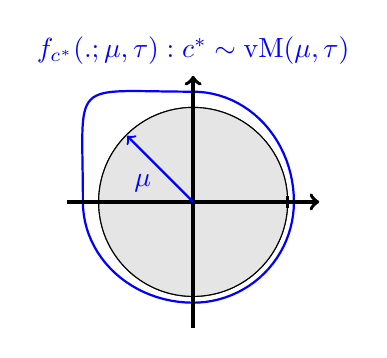
\begin{tikzpicture}[scale=0.8]
        
        \node (uni_circle) at (0,0) {};
        
        \draw[name path=circle1, black, thin] (uni_circle) circle [radius=1.5];
        \draw[name path=xaxis, black, very thick, ->] ($(uni_circle)+(-2,0)$) -- ($(uni_circle)+(2,0)$);%xaxis
        \draw[name path=yaxis, black, very thick, ->] ($(uni_circle)+(0,-2)$) -- ($(uni_circle)+(0,2)$);%yaxis
        
        \draw [name path=dist90,blue,thick,domain=0:90] plot ({1.6*cos(\x)}, {1.75*sin(\x)});
        \draw [name path=dist270,blue,thick,domain=180:270] plot ({1.75*cos(\x)}, {1.6*sin(\x)});
        \draw [name path=dist360,blue,thick,domain=270:360] plot ({1.6*cos(\x)}, {1.6*sin(\x)});
        
        \draw [name path=dist180,blue,thick,domain=90:180] ($(uni_circle)+(-1.75,0)$) .. controls +(0,2) and +(-2,0) .. ($(uni_circle)+(0,1.75)$);
        
        
        \draw[black, fill=black!10, thin] (uni_circle) circle [radius=1.5];
        \draw[black, very thick, ->] ($(uni_circle)+(-2,0)$) -- ($(uni_circle)+(2,0)$);%xaxis
        \draw[black, very thick, ->] ($(uni_circle)+(0,-2)$) -- ($(uni_circle)+(0,2)$);%yaxis
        \draw[very thick] ($(uni_circle)+(1.5,-0.1)$) -- ($(uni_circle)+(1.5,0.1)$);%1 point coordinate
        %\node at ($(uni_circle)+(1.5,-0.25)$) {$1$};
        \draw[blue, thick, ->] ($(uni_circle)$) -- ($(uni_circle)+(-1.05,1.05)$);%\mu vector
        
        \node[blue] at ($(uni_circle)+(-0.8,0.3)$) {$\mu$};
        \node[blue] at ($(uni_circle)+(0,2.4)$) {$f_{c^*}(.; \mu, \tau): c^* \sim \mbox{vM}(\mu, \tau)$};
    \end{tikzpicture}
    %\vspace{-0.2cm}
    \caption{The von Mises distribution, a distribution on the circle. The decoder uses $R\times H$ independent von Mises variables, one angle per stochastic coefficient and head.}
    \label{figure:vonMisesDist}
\end{figure}

\begin{figure*}[!htbp]
    \centering
    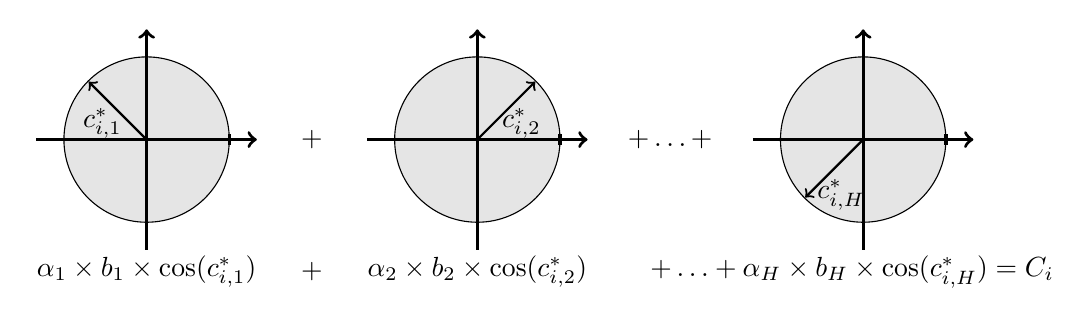
\begin{tikzpicture}[scale=0.7]
        
        \node (uni_circle1) at (0,0) {};
        
        \draw[black, fill=black!10, thin] (uni_circle1) circle [radius=1.5];
        \draw[black, very thick, ->] ($(uni_circle1)+(-2,0)$) -- ($(uni_circle1)+(2,0)$);%xaxis
        \draw[black, very thick, ->] ($(uni_circle1)+(0,-2)$) -- ($(uni_circle1)+(0,2)$);%yaxis
        \draw[very thick] ($(uni_circle1)+(1.5,-0.1)$) -- ($(uni_circle1)+(1.5,0.1)$);%1 point coordinate
        \draw[black, thick, ->] ($(uni_circle1)$) -- ($(uni_circle1)+(-1.05,1.05)$);%\mu
        \node[black] at ($(uni_circle1)+(-0.8,0.3)$) {$c^*_{i,1}$};
        
        \node at ($(uni_circle1)+ (3,0)$) {$+$};
        
        \node (uni_circle2) at (6,0) {};
        \draw[black, fill=black!10, thin] (uni_circle2) circle [radius=1.5];
        \draw[black, very thick, ->] ($(uni_circle2)+(-2,0)$) -- ($(uni_circle2)+(2,0)$);%xaxis
        \draw[black, very thick, ->] ($(uni_circle2)+(0,-2)$) -- ($(uni_circle2)+(0,2)$);%yaxis
        \draw[very thick] ($(uni_circle2)+(1.5,-0.1)$) -- ($(uni_circle2)+(1.5,0.1)$);%1 point coordinate
        \draw[black, thick, ->] ($(uni_circle2)$) -- ($(uni_circle2)+(1.05,1.05)$);%\mu
        \node[black] at ($(uni_circle2)+(0.8,0.3)$) {$c^*_{i,2}$};
        
        \node at ($(uni_circle2)+ (3.5,0)$) {$+\dots+$};
        
        
        \node (uni_circle3) at (13,0) {};
        \draw[black, fill=black!10, thin] (uni_circle3) circle [radius=1.5];
        \draw[black, very thick, ->] ($(uni_circle3)+(-2,0)$) -- ($(uni_circle3)+(2,0)$);%xaxis
        \draw[black, very thick, ->] ($(uni_circle3)+(0,-2)$) -- ($(uni_circle3)+(0,2)$);%yaxis
        \draw[very thick] ($(uni_circle3)+(1.5,-0.1)$) -- ($(uni_circle3)+(1.5,0.1)$);%1 point coordinate
        \draw[black, thick, ->] ($(uni_circle3)$) -- ($(uni_circle3)+(-1.05,-1.05)$);%\mu
        \node[black] at ($(uni_circle3)+(-0.4,-1)$) {$c^*_{i,H}$};
        
        
        %cosines sinusoidals
        \node[black] at ($(uni_circle1)+(0,-2.4)$) {$\alpha_1 \times b_1 \times \mbox{cos}(c^*_{i,1})$};
        \node[black] at ($(uni_circle1)+(3.,-2.4)$) {$+$};
        \node[black] at ($(uni_circle2)+(0,-2.4)$) {$\alpha_2 \times b_2 \times \mbox{cos}(c^*_{i,2})$};
        %\node[blue] at ($(uni_circle2)+(3,-2.4)$) {$+ \dots + $};
        \node[black] at ($(uni_circle3)+(-0.2,-2.4)$) {$+ \dots +  \alpha_H \times b_H \times \mbox{cos}(c^*_{i,H}) = C_i$};
        
        
        
    \end{tikzpicture}
    \caption{How the higher DCT coefficients are computed from $H$ sinusoidals.}
    \label{figure:vonMisesCoefficients}
\end{figure*}



\section{Extended results}\label{supp:results}
\subsection{What the relaxed decoder can express}\label{sec:res:oracle}


Table~\ref{tab:oracle} and Fig.~\ref{M-fig:oracle} show the projection bound. At $\kappa=2$, the cutoff we use for every relaxed decoder, the retained block holds 97.9\% of the energy of a run-z-scored volume, which is why the relaxation lowers the voxel error: with the minimal preprocessing of Section~\ref{supp:setup} and one 13/4 subject split, the zero-filled decoder has an RMSE of $0.556\pm0.005$ against $0.568\pm0.007$ at full resolution (five seeds). The same projection keeps only 33\% of a typical voxel's temporal variance, and the projected time course correlates with the observed one at $r=0.57$. Along $z$ the cutoff (15 coefficients) lies just below the 16 non-trivial frequencies left by the resizing of the 16-slice acquisition, so the $\kappa=2$ loss is in-plane. The energy that survives is the static, spatially smooth anatomy. The fluctuations, which are what an EEG could in principle inform, are largely above the cutoff. Any zero-filled decoder at $\kappa=2$ therefore has a brain RMSE floor of 0.205, and it cannot express two thirds of the dynamics even with perfect information. Stronger relaxations ($\kappa=4,8$) lower the ceiling further. The relaxation helps the error metric for the same reason that it limits what the EEG can contribute.

\subsection{No method is significantly better than an EEG-free predictive distribution}\label{sec:res:uq}


Table~\ref{M-tab:uq} gives the benchmark. The population template, a voxelwise Normal that never sees EEG, has a brain RMSE of 0.520, an NLL of 0.463 and a CRPS of 0.239. \textbf{No method is significantly better on any of the three} (effect sizes in Table~\ref{tab:effects}). The deep ensemble comes closest (NLL 0.393, but $p=0.23$ over subjects; CRPS 0.242; RMSE 0.526). The single-model methods all lie between NLL 0.47 and 0.55: heteroscedastic 0.522, evidential 0.513, MC dropout 0.471, stochastic spectral decoder 0.497, Flipout 0.489 (relaxed decoder) and 0.529 (full resolution), SWAG 0.549, last-layer Laplace 0.538. Their RMSE lies between 0.536 and 0.552, above the template's (CQR 0.569; the point model 0.576). The scale head matters for the stochastic spectral decoder: with the voxel head (ablation row) it has the worst NLL, CRPS and error--uncertainty correlation in the grid (NLL 0.872, $\rho=0.07$), and its error varies strongly across seeds (RMSE $0.616\pm0.083$). MC spectral dropout diverged in every seed: dropping retained DCT coefficients removes most of the volume's energy, and the network cannot compensate. The stimulus-locked template scores like the population template on this target. The own-subject oracle shows how much of the error is subject-specific anatomy (RMSE 0.053).

\begin{table}[!htbp]
	\centering
	\caption{Effect sizes for the claims of absence (run-z-score target, 17 subjects). Hodges--Lehmann estimate of the paired difference over subjects with a subject-bootstrap 95\% CI, and the $p$-value of a non-superiority test against the smallest effect size of interest $\delta$ (bold: $p<0.05$, i.e.\ an improvement of at least $\delta$ is rejected). $\Delta$NLL and $\Delta$CRPS: method minus population template ($\delta_{\mathrm{NLL}}=\sesoiNLL$, $\delta_{\mathrm{CRPS}}=\sesoiCRPS$, 5\% of the template--oracle gap; negative is better). $\Delta r$: median voxel temporal $r$ with the real EEG minus with another subject's EEG ($\delta_r=0.05$).}
	\label{tab:effects}
	\setlength{\tabcolsep}{3pt}
	\resizebox{\textwidth}{!}{%
	\begin{tabular}{lcccccc}
		\toprule
		Method & $\Delta$NLL vs template & $p_{\mathrm{ns}}$ & $\Delta$CRPS vs template & $p_{\mathrm{ns}}$ & $\Delta r$ real $-$ swap & $p_{\mathrm{ns}}$\\
		\midrule
		\tabinput{tables/effects}
		\bottomrule
	\end{tabular}}
\end{table}

Table~\ref{tab:effects} turns these non-significant differences into bounds. For every single-model method, an NLL improvement over the template of at least $\delta_{\mathrm{NLL}}=\sesoiNLL$ is rejected ($p\le0.03$), and so is a CRPS improvement of at least $\delta_{\mathrm{CRPS}}$ for every method. The deep ensemble is the exception: its NLL difference from the template is $-0.038$ with a 95\% CI of $[-0.175, 0.021]$, so a meaningful improvement can be neither shown ($p=0.23$) nor excluded ($p=0.14$). Most of its advantage comes from mixing: the five-member mixture improves the NLL of its own members by $0.129$ $[0.120, 0.138]$, while their mean single-member NLL is $0.522$, worse than the template.

\paragraph{The usual UQ diagnostics do not separate the models from the template.} The template's own 90\% intervals cover 84\% of test voxels. The networks' likelihood intervals cover 76--89\% and CQR's unconformalized quantiles 67\% (Fig.~\ref{M-fig:reliability}, left), with SWAG and the heteroscedastic, evidential and Laplace heads the most overconfident. Per-voxel conformal calibration on two held-out subjects brings every method, the template included, to 72--79\% at the nominal 90\% (template 72\%) (Fig.~\ref{M-fig:reliability}, right). Conformalization lowers the template's coverage from 0.84 to 0.72: the per-voxel quantiles of two calibration subjects are narrower than the spread of new subjects. The shortfall is the same for all methods. It reflects between-subject heterogeneity, which two calibration subjects cannot represent, and not a property of any method. Cross-conformal calibration over all non-test subjects (Section~\ref{sec:res:crossconformal}) tests this directly. The correlation between predictive spread and error is \emph{highest for the template} ($\rho=0.52$, against 0.47--0.51 for the networks that trained normally), and its AUSE (0.106) is matched only by the ensemble (0.105). The template's spread is large where anatomy varies across subjects (edges, ventricles, the boundary of the field of view), and so are everyone's errors. A model that reproduces that spread, as all of them do, gets a good sparsification curve without using the EEG.



\subsection{No method's prediction or uncertainty depends on subject-specific EEG}\label{sec:res:nulls}
Fig.~\ref{fig:nulls} shows the temporal correlation of every method under the real EEG and the two nulls. All are below 0.016, against 0.160 for the stimulus-locked template without EEG ($p=1$ for every method against it). Of the methods in Table~\ref{M-tab:uq}, only the deep ensemble exceeds the shift null ($r=0.015$ vs $-0.003$, $p=0.049$). Its difference from the shift null is $0.015$ $[-0.002, 0.035]$, and it does not exceed the swap null ($0.009$, $p=0.29$); no other method exceeds either null on $r$. Against the swap null, an EEG-specific gain of at least $\delta_r=0.05$ is rejected for every method ($p<0.001$, Table~\ref{tab:effects}). On the run-level scores, MC dropout ($p<0.001$ on centred $R^2$ and NLL), SWAG ($p=0.03$, $p=0.01$), the stochastic spectral decoder ($p=0.04$ on centred $R^2$) and CQR ($p=0.03$ on the pooled detrended $r$) are better with the real EEG than with the shifted EEG. None of them is better than with another subject's EEG ($p\ge0.27$; Supplementary Table~\ref{tab:nulls_full}). What these models pick up is locked to the run and its shared task timing, not to the subject's EEG. The predictive distribution itself does not change with the EEG either: the NLL under the shift null differs from the real NLL by at most 0.003 for every method.

\paragraph{The predicted uncertainty does not depend on the EEG at all.}
\begin{table}[!htbp]
	\centering
	\caption{Does the predictive spread depend on the EEG? Mean over the 5 folds (seed 2; the ensemble over its 5 members), test subjects, brain mask. Temporal/spatial: variance of the predictive SD $\sigma$ over time within voxels relative to its variance across voxels. $\rho_\sigma$: spatial correlation of the time-averaged $\sigma$ map with the real EEG and with the shift or swap null. $W_2^{\sigma}$ and $W_2^{\mu}$: spread and mean terms of the squared 2-Wasserstein distance between the real and swap-null predictive distributions (moment-matched), relative to the average predictive variance. Last two columns: Spearman correlation of $\sigma$ with the anatomical component of the error (its temporal mean, across voxels) and with the temporal component (within voxels, over time).}
	\label{tab:uqdep}
	\setlength{\tabcolsep}{3pt}
	\resizebox{\textwidth}{!}{%
	\begin{tabular}{lccccccc}
		\toprule
		Method & temporal/spatial & $\rho_\sigma$ shift & $\rho_\sigma$ swap & $W_2^{\sigma}$ swap & $W_2^{\mu}$ swap & $\rho(\sigma, |e_{\mathrm{anat}}|)$ & $\rho(\sigma, |e_{\mathrm{temp}}|)$\\
		\midrule
		\tabinput{tables/uq_dependence}
		\bottomrule
	\end{tabular}}
\end{table}


Table~\ref{tab:uqdep} answers the title question directly. For every method the predictive SD is a fixed map: its variance over time is $10^{-6}$ to $10^{-3}$ of its variance across voxels, and the maps obtained with the real EEG, with the shifted EEG and with another subject's EEG correlate at $1.000$. The distance between the real and null predictive distributions comes almost entirely from their means; the spread term is $10^{-6}$ to $10^{-3}$ of the predictive variance. The spread tracks the anatomical component of the error ($\rho\approx0.5$) and not its temporal component ($\rho\le0.02$). The uncertainty these methods report is an anatomical map of where subjects differ, identical whatever EEG is given (Fig.~\ref{M-fig:volumes}). For the stochastic spectral decoder the epistemic part is almost absent: trained by maximum likelihood without a prior, its noise parameters shrink until the epistemic variance is $4\times10^{-6}$, against an aleatoric variance of $0.26$, so its reported uncertainty is essentially that of its aleatoric head.

\subsection{Coverage with all subjects as calibration}\label{sec:res:crossconformal}
The under-coverage of Fig.~\ref{M-fig:reliability} is a calibration-sample effect (Table~\ref{tab:crossconf}). With the out-of-fold scores of all 16 other subjects, the per-voxel intervals cover 88--89\% at the nominal 90\% and the global ones 90\%, although single subjects still fall to 72--83\%. Conformal calibration over subjects works; it simply needs more than two of them. It does not, however, make the intervals informative about the EEG: they are built on the same static spread.



The same conclusion holds voxel by voxel (Fig.~\ref{M-fig:sigmaps}). The sensitive network beats the time-shifted EEG in almost half of the brain voxels of the slab, but another subject's EEG in fewer voxels than chance, and the EEG-free stimulus-locked template beats the network almost everywhere.

\subsection{The ECG and a minimal preprocessing}\label{sec:res:controls}
A network that sees only the ECG lead scores almost like one that sees 63 EEG channels (Table~\ref{tab:controls}). Paired over subjects, the EEG input does not improve the NLL ($-0.004$ $[-0.076, 0.049]$) and raises the temporal correlation by $0.010$ $[0.002, 0.017]$ ($p=0.012$), a fifth of the smallest effect of interest. With the minimal preprocessing, the temporal correlation exceeds the shift null ($p=0.007$) but not the swap null ($p=0.46$), and the NLL is much worse (0.792). The extra input (the ECG lead and mirrored high-frequency bins) adds run-locked signal and over-confidence, not information about the subject.

\subsection{On the dynamics alone, the networks predict no change}\label{sec:res:dynamics}
Removing the anatomy makes the question direct: can the network predict how each voxel changes over time? Table~\ref{tab:dynamics} says no. At every relaxation and at full resolution the networks converge to the no-change prediction: median voxel $r\le0.005$, never above the shift ($p\ge0.07$) or swap ($p\ge0.11$) null, and an NLL slightly worse than the no-change template. The dynamics are predictable, however: the stimulus-locked template, which only knows when the motor imagery blocks occur, reaches a median voxel $r$ of 0.163. The networks do not learn even that from the EEG. Once the task-locked response is removed (residual target), nothing predictable is left for any method ($r\approx0$).

\subsection{A positive control: the networks miss a signal a linear model recovers}\label{sec:res:positive}

A negative result needs a pipeline that could have detected a positive one. We therefore inject a signal that is, by construction, a linear function of the models' own EEG input (Table~\ref{M-tab:positive}). A closed-form ridge on the same input window recovers it at every strength: $r=0.18$ at $s=0.1$, $0.34$ at $s=0.3$ and $0.59$ at $s=1$, against ceilings of $0.30$, $0.48$ and $0.71$, with both nulls near zero ($p<10^{-4}$ over subjects for each). The heteroscedastic backbone, the base of most UQ methods in Table~\ref{M-tab:uq}, does not recover it at any strength.

The ablation ladder locates the loss. The same linear map and MLP on the same features recover the signal when trained as a regression ($r=0.49$ and $0.54$ at $s=1$; $0.09$ and $0.12$ at $s=0.1$), and lose most or all of it when trained with the deep models' loop ($0.20$ and $0.01$ at $s=1$). The backbone behaves the same way: with a point $L_1$ loss it recovers the signal ($r=0.48$ at $s=1$), and so does the heteroscedastic head when the learning rate is lowered to $10^{-4}$ ($r=0.49$). The architecture is capable; what makes it blind to its input is training a heteroscedastic likelihood at the searched learning rate. This is a known failure mode of heteroscedastic regression, in which a learned variance absorbs the residual and the mean stops fitting \citep{seitzer2022pitfalls}. Here it produces calibrated, sharp-looking uncertainty from models that ignore the EEG.

The positive control also fixes the reading of the main negative result. Trained with the recipes that recover the injected signal, the networks on the real fluctuation target reach a median voxel $r$ of $0.035$ (point loss) and $0.030$ (heteroscedastic, learning rate $10^{-4}$) in native space and $0.066$ on registered volumes. That is above the time-shift null ($p=0.022$, $0.010$ and $<0.001$) but not above the subject-swap null ($0.030$, $0.025$ and $0.059$; $p\ge0.37$), exactly as for the linear probe below. On the run z-score the sensitive heteroscedastic network is worse than the template (NLL $0.877$ vs $0.463$), and its predicted spread is still a static map that does not change with the EEG (Table~\ref{tab:uqdep}, last row). Models that can see an EEG-coupled signal find only what is locked to the shared task timing.

The same ridge, applied to the real fluctuation target without injection, predicts the voxel time courses slightly better than the shift null (median $r=0.024$ vs $-0.008$, $p=0.013$; on registered volumes $0.081$ vs $-0.021$, $p=0.005$) but not better than the swap null ($0.018$, $p=0.31$; registered $0.063$, $p=0.18$). What a sensitive linear model finds in these data at the voxel level is locked to the shared task timing, not specific to the subject's EEG.

\subsection{Registered volumes}\label{sec:res:registered}
Registration does not change the conclusions (Table~\ref{tab:registered}). On registered volumes every method has a higher NLL than the population template computed on the same volumes (the ensemble comes closest, $0.948$ vs $0.795$), and only the heteroscedastic network on the fluctuation target exceeds the shift null, by a negligible margin ($r=0.006$, $p<0.001$); no method exceeds the swap null. Registration does make the dynamics far more predictable without EEG: the stimulus-locked template reaches a median voxel $r$ of $0.46$ on the run z-score and $0.50$ on the fluctuation target, against $0.16$ in native space, because the task response now falls on the same voxels in every subject. The networks learn none of it. The linear probe on registered fluctuations reaches $r=0.081$, above the shift null ($p=0.005$) but not the swap null ($0.063$, $p=0.18$), as in native space.

\subsection{At the scale of a region, heart rate predicts as much as the EEG}\label{sec:res:ridge}
\begin{table}[!htbp]
	\centering
	\caption{ROI ridge arm: lagged features predicting the sensorimotor ROI BOLD (registered volumes; Section~\ref{sec:ridge}). $r$: mean test correlation over subjects. Block: the HRF-convolved block design alone on the raw ROI time course. $p_{>\mathrm{block}}$: paired Wilcoxon over subjects. Sig.: subjects whose $r$ exceeds their 100 IAAFT surrogates ($p<0.05$), with the binomial group $p$. Swap: the same fitted model scored on another subject's features (mean $r$, and the paired $p$ of real $>$ swap).}
	\label{tab:ridge}
	\small
	\begin{tabular}{lccccccc}
		\toprule
		Features, target & $n$ & $r$ & block $r$ & $p_{>\mathrm{block}}$ & sig. & $p_{\mathrm{binom}}$ & swap $r$ ($p$)\\
		\tabinput{tables/ridge}
		\bottomrule
	\end{tabular}
\end{table}





The ridge arm asks whether the voxel-level negative result reflects the data or the deep, voxel-level setting (Tables~\ref{tab:ridge} and~\ref{M-tab:nested}, Fig.~\ref{M-fig:ridge}). \emph{Within subjects}, with the task regressed out, 7 of 17 subjects beat their surrogates with the EEG, 3 with ECG band power and 7 with heart rate, and none of the models beats the block design ($p\ge0.19$). \emph{Across subjects} the EEG ridge looks like a success. With the task regressed out it reaches $r=0.243$, 13 of 17 subjects beat their surrogates (binomial $p<0.001$), it beats the same model scored on another subject's EEG ($r=0.053$, $p<0.001$), and it survives motion regression ($r=0.240$). It does not beat the block design once the task is regressed out ($r=0.152$, $p=0.066$), although it does on the raw ROI time course ($r=0.264$, $p=0.028$). By the criteria of the field, and by Mehta et al.'s, it would count as EEG-to-fMRI prediction.

It is not specific to the EEG. Heart rate alone, from the in-scanner ECG, predicts the same ROI as well ($r=0.268$, 13 of 17 subjects; EEG not better than heart rate, paired $p=\ridgeEEGvsHR$). Across subjects, in nested models, the EEG adds nothing to heart rate and motion: the held-out $R^2$ is $0.065$ without and $0.064$ with it ($\Delta R^2=-0.001$, $p=0.50$ for a gain), and adding ECG band power does not change this ($\Delta R^2=0.010$, $p=0.36$). Within subjects the EEG adds a small amount to heart rate and motion ($\Delta R^2=0.028$, $p=0.044$, uncorrected), which does not survive the inclusion of ECG band power ($\Delta R^2=0.013$, $p=0.15$). And the EEG still carries the heart: after pulse-artefact correction, 20\% of the EEG band-power features correlate with heart rate at $|r|>0.2$, against 1.7\% when heart rate is shifted by at least 30\,s ($p<0.001$ over subjects). A subject-specific physiological signal predicts the sensorimotor BOLD across subjects as well as the EEG does, and what the EEG adds beyond it is at most small.

\subsection{The pipeline and test of Mehta et al.}\label{sec:res:mehta}
Applied as published, Mehta et al.'s test supports EEG-to-BOLD prediction in our data too (Table~\ref{tab:mehta}; 16 subjects, sub-xp202 has no EEG export for one run). On the trial-evoked signal, the sparse group lasso reaches $r=0.182$ within runs and $0.155$ across runs, 8 of 16 subjects beat their 100 IAAFT surrogates in each design (binomial $p<0.001$), and it beats both of their reference models (FDR-corrected $p\le0.046$). On the trial-by-trial signal it is weaker ($r=0.078$ and $0.045$; 8 and 3 of 16) and better than their C3/C4 reference model in neither design. Our counts are lower than their 13 of 15. Our two runs come from one session rather than two sessions two weeks apart, and our ROI is anatomical rather than a functional network, so the settings are not identical.

The same pipeline and test, fitted to the ECG lead alone, do nearly as well: $r=0.149$ and $0.127$ (9 and 6 of 16) on the trial-evoked signal, and better than the EEG on the trial-by-trial signal, $0.120$ and $0.063$ (10 and 6 of 16). A surrogate test over the BOLD, however carefully run, establishes that a model predicts better than chance. It does not establish that the predictive information is neural, and in simultaneous EEG--fMRI the cardiac signal is the obvious alternative.

\subsection{Replication on CHUR-XP1}\label{sec:res:xp1}
\begin{table}[!htbp]
	\centering
	\caption{CHUR-XP1 replication (ds002336 motor localizer, 9 subjects, registered volumes, EEG aligned to the scanner pulses; five subject folds). Top: the main configurations on the run z-score against the EEG-free population template (NLL with the one-sided $p$ of being better; CRPS), median voxel temporal $r$ with $p$ against the shift and swap nulls, the stimulus-locked template's $r$, and per-voxel conformal coverage at 90\%. Middle: positive control, injected signal at $s=1$ (ceiling 0.71), median $r$ in the injected box with the shift and swap nulls in brackets. Bottom: ROI ridge across subjects, task regressed out, with surrogate and swap tests and the nested model. The fold with a single test subject has no swap null.}
	\label{tab:xp1}
	\setlength{\tabcolsep}{3pt}
	\resizebox{\textwidth}{!}{%
	\begin{tabular}{lccccccc}
		\toprule
		Method & NLL vs template ($p$) & CRPS vs template & $r$ & $p_{>\mathrm{shift}}$ & $p_{>\mathrm{swap}}$ & $r$ locked & Conf$_{90}$\\
		\midrule
		\tabinput{tables/xp1_uq}
		\bottomrule
	\end{tabular}}

	\vspace{0.6em}
	\begin{tabular}{lc}
		\toprule
		Positive control ($s=1$) & $r$ in box (shift, swap)\\
		\midrule
		\tabinput{tables/xp1_positive}
		\bottomrule
	\end{tabular}
	\hspace{1em}
	\begin{tabular}{lccccc}
		\toprule
		ROI ridge features & $n$ & $r$ & sig. & $p_{\mathrm{binom}}$ & swap $r$ ($p$)\\
		\midrule
		\tabinput{tables/xp1_ridge}
		\bottomrule
	\end{tabular}
\end{table}
We repeated the main analyses on CHUR-XP1 (Table~\ref{tab:xp1}). Its motor-localizer run has a 2-s TR, near whole-brain coverage and an EEG export that starts before the first scanner pulse, so every EEG window was aligned to its pulse; one subject without a motor-localizer EEG export was excluded.

The voxel-level results replicate. No model's temporal prediction exceeds the subject-swap null, while the EEG-free stimulus-locked template reaches a median voxel $r$ of $0.63$. The heteroscedastic network with the lower learning rate exceeds the time-shift null ($r=0.053$, $p=0.049$) but not the swap null, as on CHUR-XP2. One result differs: two methods have a lower NLL than the template, the deep ensemble ($0.294$ vs $0.653$, $p=0.004$; Hodges--Lehmann $-0.36$ $[-0.55, -0.15]$) and the stochastic spectral decoder ($0.400$, $p=0.020$), although no method has a lower CRPS (ensemble $0.207$ vs $0.197$) or RMSE, and their predictions carry nothing beyond the swap null. With six or seven training subjects per fold the template's voxelwise spread is poorly estimated, and mixtures over seeds or noise samples are more forgiving on the likelihood; on CHUR-XP2 most of the ensemble's advantage came from the mixture itself (Section~\ref{sec:res:uq}). We read it as a calibration effect, not as EEG information. The ensemble's NLL improves on its own members by $0.17$ $[0.15, 0.18]$, almost half its distance from the template. With 8 or 9 subjects the equivalence bounds are wider than on CHUR-XP2: an EEG-specific gain of $\delta_r=0.05$ over the swap null is rejected for the heteroscedastic network, the stochastic spectral decoder and the ensemble ($p=0.004$, $0.020$ and $0.012$) but cannot be excluded for the point-loss model and the heteroscedastic network with the lower learning rate ($p=0.055$ and $0.19$). The predicted uncertainty is again a static map: for the heteroscedastic network, with either learning rate, its temporal variance is $10^{-5}$ of its spatial variance or less, and the maps under the real, shifted and swapped EEG correlate at $1.000$.

The positive control replicates. The backbone trained with a point loss recovers the injected signal ($r=0.368$; nulls $-0.044$ and $0.113$), the heteroscedastic backbone does not ($-0.016$, against a swap null of $0.007$), and the linear probe recovers it best ($0.625$). The point-loss model on the real fluctuations exceeds the time-shift null ($r=0.059$, $p=0.014$) but not the swap null ($0.051$, $p=0.37$), as on CHUR-XP2.

At the region level the direction replicates with less power. Across subjects the EEG ridge predicts the motor ROI with the task regressed out ($r=0.172$, 7 of 9 subjects, beyond the swap null), and heart rate also predicts it ($r=0.137$, 4 of 9). Here the EEG is numerically ahead of heart rate (paired $p=0.18$), but adding the EEG to heart rate and motion does not improve the held-out fit ($\Delta R^2=-0.005$, $p=0.54$). The cardiac content of the EEG is larger than on CHUR-XP2: 56\% of the EEG band-power features correlate with heart rate at $|r|>0.2$, against 22\% with a shifted heart rate ($p=0.002$). The in-scanner ECG is also noisier (up to 20\% of RR intervals implausible in one subject), which makes heart rate a weaker confound model here.



\begin{table}[htbp]
	\centering
	\caption{Oracle bound of the DCT relaxation on CHUR-XP2 (Section~\ref{sec:oracle}), mean over 17 subjects. The relaxation factor $\kappa$ divides each axis of the $64\times64\times30$ volume. The columns give the retained block, the number of predicted coefficients, the fraction of volume energy kept, the brain RMSE floor of any relaxed decoder on the run-z-scored target, and the median over brain voxels of the temporal variance kept and of the correlation between the projected and observed time courses. All relaxed decoders in Table~\ref{M-tab:uq} use $\kappa=2$.}
	\label{tab:oracle}
	\small
	\setlength{\tabcolsep}{4pt}
	\begin{tabular}{lcrcccc}
		\toprule
		$\kappa$ & block & coef. & energy (\%) & RMSE floor & temp.\ var.\ (\%) & temp.\ $r$ \\
		\midrule
		\tabinput{tables/oracle}
		\bottomrule
	\end{tabular}
\end{table}

\begin{figure}[htbp]
	\centering
	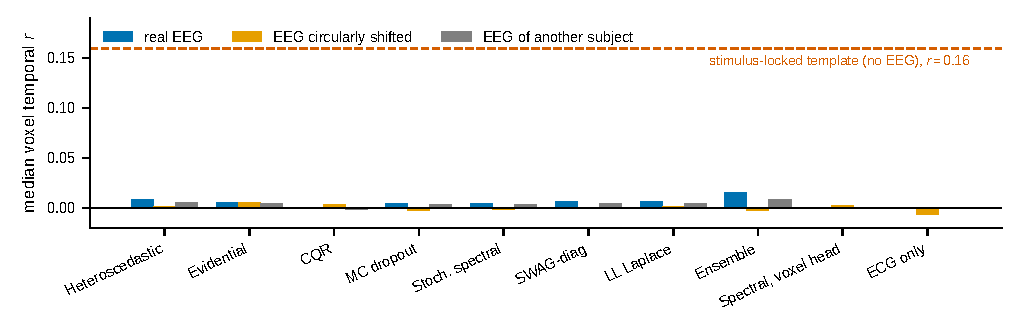
\includegraphics[width=\textwidth]{figures/nulls.pdf}
	\caption{Median voxel temporal correlation between predicted and observed time courses (run-z-score target), with the real EEG, the EEG circularly shifted by $\ge30$\,s, and the EEG of another test subject. The dashed line is the EEG-free stimulus-locked template.}
	\label{fig:nulls}
\end{figure}

\begin{table}[htbp]
	\centering
	\caption{Empirical coverage of the per-voxel split-conformal 90\% interval on test subjects, mean [minimum] over the 17 subjects (seed 2; ensemble over its members), calibrated on the fold's two calibration subjects or cross-conformally on the out-of-fold scores of all 16 other subjects; last column: one global quantile, cross-conformal.}
	\label{tab:crossconf}
	\small
	\begin{tabular}{lccc}
		\toprule
		Method & 2 subjects, per voxel & 16 subjects, per voxel & 16 subjects, global\\
		\midrule
		\tabinput{tables/crossconf}
		\bottomrule
	\end{tabular}
\end{table}

\begin{table}[htbp]
	\centering
	\caption{Input controls for the heteroscedastic relaxed decoder (run-z-score target): the EEG input of Table~\ref{M-tab:uq}, the ECG lead alone, and a minimal preprocessing (all 64 channels including ECG, z-scored across channels, STFT bins beyond Nyquist). $p$: one-sided paired Wilcoxon over subjects for median voxel $r$ above the shift and swap nulls.}
	\label{tab:controls}
	\small
	\begin{tabular}{lccccc}
		\toprule
		Input & RMSE & NLL & median $r$ & $p_{r>\mathrm{shift}}$ & $p_{r>\mathrm{swap}}$\\
		\midrule
		\tabinput{tables/controls}
		\bottomrule
	\end{tabular}
\end{table}

\begin{table}[htbp]
	\centering
	\caption{Fluctuation targets (static anatomy removed; heteroscedastic decoder at several relaxations and at full resolution). Median voxel temporal $r$ with $p$-values against the shift and swap nulls; NLL of the model and of the EEG-free no-change template; median voxel $r$ of the EEG-free stimulus-locked template for the same target.}
	\label{tab:dynamics}
	\small
	\begin{tabular}{lcccccc}
		\toprule
		Decoder & median $r$ & $p_{r>\mathrm{shift}}$ & $p_{r>\mathrm{swap}}$ & NLL & NLL template & $r$ stimulus-locked \\
		\tabinput{tables/dynamics}
		\bottomrule
	\end{tabular}
\end{table}

\begin{table}[htbp]
	\centering
	\caption{The main configurations on registered, motion-corrected volumes (MNI, Section~\ref{supp:setup}), 17 test subjects. NLL and CRPS of the method and of the EEG-free population template on the same volumes, with the one-sided Wilcoxon $p$ of the method being better; median voxel temporal $r$ with $p$ against the shift and swap nulls; $r$ of the EEG-free stimulus-locked template; per-voxel conformal coverage at 90\%.}
	\label{tab:registered}
	\setlength{\tabcolsep}{3pt}
	\resizebox{\textwidth}{!}{%
	\begin{tabular}{llcccccccccc}
		\toprule
		Target & Method & NLL & NLL tmpl & $p$ & CRPS & CRPS tmpl & $r$ & $p_{>\mathrm{shift}}$ & $p_{>\mathrm{swap}}$ & $r$ locked & Conf$_{90}$\\
		\midrule
		\tabinput{tables/registered}
		\bottomrule
	\end{tabular}}
\end{table}

\begin{table}[htbp]
	\centering
	\caption{Replication of the pipeline and statistical test of \citet{mehta2025eegbold} on CHUR-XP2 (Section~\ref{sec:mehta}): sparse group lasso on lagged Morlet relative power, somatomotor ROI. $r$: mean test correlation over subjects (averaged over the two folds). Sig.: subjects whose $r$ exceeds their 100 IAAFT surrogates ($p<0.05$, $p=\#\{r_{\mathrm{null}}\ge r\}/N$), with the binomial group $p$. SMR and MUC: their reference models, with the Benjamini--Hochberg-corrected one-sided Wilcoxon $p$ of the sparse group lasso being better.}
	\label{tab:mehta}
	\small
	\setlength{\tabcolsep}{4pt}
	\resizebox{\textwidth}{!}{%
	\begin{tabular}{lcccccccc}
		\toprule
		Features, condition, split & $n$ & $r$ & sig. & $p_{\mathrm{binom}}$ & $r_{\mathrm{SMR}}$ & $p_{>\mathrm{SMR}}$ & $r_{\mathrm{MUC}}$ & $p_{>\mathrm{MUC}}$\\
		\midrule
		\tabinput{tables/mehta}
		\bottomrule
	\end{tabular}}
\end{table}





\begin{table}[h]
	\centering
	\caption{All EEG-null comparisons on the run-z-score target. Median voxel temporal $r$ with the real EEG, the shift null and the swap null; one-sided paired Wilcoxon $p$ over 17 subjects for real $>$ null on the pooled detrended correlation and the centred $R^2$ of the voxel time courses within the brain mask; and the NLL difference real $-$ shift with its $p$ (real $<$ shift). Bold: $p<0.05$. A method that beats the shift but not the swap null has learned something locked to the run or task timing, not the subject's EEG.}
	\label{tab:nulls_full}
	\setlength{\tabcolsep}{3pt}
	\resizebox{\textwidth}{!}{%
	\begin{tabular}{lcccccccc}
		\toprule
		& \multicolumn{3}{c}{median voxel $r$} & \multicolumn{2}{c}{pooled detrended $r$} & \multicolumn{2}{c}{centred $R^2$} & \\
		\cmidrule(lr){2-4}\cmidrule(lr){5-6}\cmidrule(lr){7-8}
		Method & real & shift & swap & $p_{>\mathrm{shift}}$ & $p_{>\mathrm{swap}}$ & $p_{>\mathrm{shift}}$ & $p_{>\mathrm{swap}}$ & $\Delta$NLL vs shift ($p$)\\
		\midrule
		\tabinput{tables/nulls_full}
		\bottomrule
	\end{tabular}}
\end{table}


\section{Extended discussion}\label{supp:discussion}
\paragraph{Calibration is not informativeness.} A predictive distribution can be calibrated, sharp enough to rival a naive baseline and correlated with its own errors without using its input. In EEG-to-fMRI synthesis this is the default: the target is dominated by anatomy that is shared across subjects, and anatomical variability determines both where errors occur and where any reasonable model is uncertain. All eleven methods learn this structure, and so does the EEG-free template, which none of them beats significantly. Their uncertainty is a fixed anatomical map that does not move with the EEG. Had we reported only NLL, PICP, Spearman and AUSE, as is common in UQ papers, the ensemble, MC dropout and the stochastic spectral decoder would have looked like successful uncertainty quantification.

\paragraph{Heteroscedastic training can blind a synthesizer to its input.} The positive control shows that the problem is not only the data. A heteroscedastic likelihood lets a network explain a residual either by moving its mean or by widening its variance. When the input is weakly informative and the learning rate is high, widening wins, and the mean stops fitting \citep{seitzer2022pitfalls}. In our setting this turned a backbone that can recover an injected EEG signal ($r=0.48$ with a point loss) into one that cannot ($r\approx0$), while its NLL, coverage and sparsification remained respectable. Every UQ method built on that solution (heteroscedastic, Laplace, SWAG, ensembles) inherits the blindness. This is the strongest argument for positive controls in UQ evaluation: a method's calibration says nothing about whether it can see a signal that is there.

\paragraph{What the EEG predicts, and what it does not.} Models that can see an EEG-coupled signal still find little in the real data. At the voxel level, the point-loss decoder and a linear probe on the same input exceed the time-shift null only through the shared task timing; neither exceeds the subject-swap null. At the region level, a lagged linear model predicts motor BOLD across subjects as convincingly as any published result. But heart rate predicts the same region as well, the EEG adds nothing to heart rate and motion across subjects and at most a small within-subject increment that does not survive the ECG, and the EEG still contains cardiac signal after pulse-artefact correction. The simplest reading is that the region-level prediction is physiological: heart-rate fluctuations drive BOLD changes through cerebral blood flow, and they enter the EEG through residual pulse artefacts and autonomic covariation. This does not mean that EEG--BOLD coupling is absent. Alpha and mu/beta power covary with BOLD in specific networks \citep{goldman2002simultaneous,laufs2003eeg}. It means that in this dataset a predictive model cannot separate that coupling from physiology, and that a surrogate test over the BOLD, including the careful test of Mehta et al., cannot either. Region-level synthesis models report cross-subject correlations of a similar size on other datasets \citep{li2024neurobolt}; we suggest that they report heart-rate and motion models, and nested comparisons, alongside them.

\paragraph{Practices.} The protocol is general, and we suggest the following for EEG-to-fMRI synthesis and similar cross-modal tasks:
\begin{enumerate}
	\item report proper scores (NLL, CRPS) of an EEG-free predictive distribution next to every model, including a stimulus-locked one when the task timing is shared;
	\item evaluate every trained model under a temporal-shift null and a subject-swap null, and claim EEG-specific information only above the swap null;
	\item test whether the predicted uncertainty changes with the input, not only whether it is calibrated;
	\item include a positive control: inject a known input-coupled signal and show that the model, trained exactly as reported, recovers it;
	\item fit physiological confound models (heart rate from the ECG, head motion) with the same pipeline, and test the EEG's increment over them in nested models;
	\item split by subject, calibrate conformal intervals over many subjects (cross-conformally if needed), and report coverage per subject;
	\item check the EEG--fMRI alignment from the scanner markers and the spectral bins against the Nyquist frequency, register the volumes from the scanner's world coordinates when the field of view is partial, and check every registration visually;
	\item report effect sizes with confidence intervals and a smallest effect of interest for every claim of absence.
\end{enumerate}

\paragraph{Limitations.} The analyses use two motor-imagery datasets from one laboratory, with 17 and 9 subjects and block designs; the region-level confound result is weaker on the smaller, noisier-ECG cohort. Subject-level tests with $n=17$ have limited power, but the equivalence tests bound the effects we could have missed (Table~\ref{tab:effects}). The positive control injects a linear, spatially fixed signal; real EEG--BOLD coupling may be nonlinear and spatially specific, and we test sensitivity, not the full range of plausible couplings. The backbone's architecture was fixed by the original neural architecture search, and the UQ methods share its searched learning rate. A lower learning rate rescues the heteroscedastic head on the positive control, but we did not retune and rerun every method, and the conclusions about each method apply to it as configured. Heart rate was derived from the in-scanner ECG, which contains gradient residuals; at most 9\% of RR intervals per subject were implausible and interpolated. Respiration was not recorded and could account for part of what we attribute to heart rate. Both arms normalize each subject with its own run (transductive normalization), as is standard in this literature; the EEG-free references are scored on the same normalized data. Finally, the registered-volume analyses used a corrected registration, and the native-space analyses inherit the geometry of the original backbones (Section~\ref{sec:res:registered}).



\printbibliography

\end{document}
